\section{AlexNet}

\href{http://papers.nips.cc/paper/4824-imagenet-classification-with-deep-convolutional-neural-networks.pdf}{AlexNet}
\footnote{Krizhevsky, A., Sutskever, I., Hinton, G. E. (2012). Imagenet classification with deep convolutional neural networks. In Advances in neural information processing systems (pp. 1097-1105).}  popularized convolutional neural networks (CNNs) after winning the \href{http://image-net.org/challenges/LSVRC/2012/index}{ImageNet ILSVRC 2012} challenge with a huge margin to the runner-up.
It has been observed that the filters in the first layer of a CNN usually resemble Gabor filters.
This question explores this idea.

\begin{enumerate}
\item \points{5} \textbf{Weight visualization}

  Download the pre-trained AlexNet weights here:  \url{http://www.vlfeat.org/matconvnet/models/imagenet-caffe-alex.mat}.
  Load the weights of the first layer on MATLAB by doing:
  \begin{lstlisting}[language=matlab]
    model = load('imagenet-caffe-alex.mat');
    weights = model.layers{1}.weights{1};
  \end{lstlisting}
  You should obtain a $11\times 11\times 3\times 96$ tensor.
  This corresponds to 96 filters with dimensions $11\times 11$ and 3 channels (B, G, R).
  Plot the filters arranged in a $12\times 8$ grid. \emph{Hint: normalize the filters to be between 0 and 1 for better visualization.}

  Select, from the 96 filters, examples of filters that can and that cannot be approximated with the real part of a 2D Gabor (as produced by \verb|gaborFilter2D.m|).
  Explain your answer.

  Note that, since the filters are applied convolutionally, we don't care much about the spatial position, i.e., an off-centered filtered with small support is equivalent to its centered version.

\item \points{7} \textbf{Approximating filters with Gabors}
    \begin{figure}[ht!]
      \begin{center}
        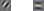
\includegraphics[width=0.4\textwidth]{images/alexnet.png}
      \end{center}
      \caption{\label{fig:alexnet} A couple of AlexNet filters.}
    \end{figure}

  Consider the two filters from Figure~\ref{fig:alexnet}.
  Approximate them by $11\times 11$ 2D Gabor filters.
  Show your approximations and the parameters chosen.

  In AlexNet, each of the $11\times 11\times 3\times 96$ weights of the first layer have to be learned.
  If we were the replace the first layer of AlexNet with a bank of $96$ Gabor filters, how many parameters would have to be learned?
\end{enumerate}



%%% Local Variables: 
%%% mode: latex
%%% TeX-master: "../hw3"
%%% End: 
